\Chapter{Operations Involving the Integers}
\Lettrine[loversize=0.1,nindent=0pt]{There} is not much difference between the natural numbers and the integers. The naturals and integers are numbers we can add, multiply, and exponentiate. The distinguishing characteristic that the integers have over the natural numbers is the operation of subtraction, which we will also look at in this chapter.

\section{Addition}
Integer addition is nothing special. Consider the numbers 4 and 3 represented by the shifts $(6,2)$ and $(5,2)$ respectively. What happens when we add them? Visually, this means that we can apply the shifts in the following order:
\begin{enumerate}
    \item Shift rightward by 6.
    \item Shift leftward by 2.
    \item Shift rightward by 5.
    \item Shift leftward by 2.
\end{enumerate}
\begin{figure}[H]
    \centering
    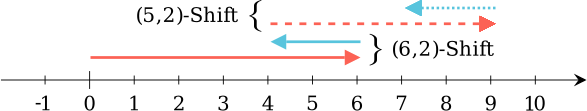
\includegraphics[width=9cm]{images/part-2/operations-on-integers/addition-number-line_separate.png}
    \caption{Adding 4 and 3, As Two Separate Shifts}
\end{figure}

But one notices that we can combine the rightward and leftward shifts together. In other words, we just need to apply the following shifts:
\begin{enumerate}
    \item Shift rightward by $6 + 5$.
    \item Shift leftward by $2 + 2$.
\end{enumerate}
\begin{figure}[H]
    \centering
    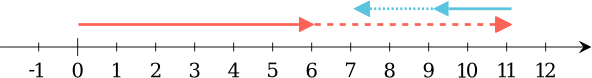
\includegraphics[width=9cm]{images/part-2/operations-on-integers/addition-number-line_combined.png}
    \caption{Adding 4 and 3, As A Combined Shift}
\end{figure}

This leads us to define integer addition as follows.
\begin{definition}[Addition (Integers)]
    The \term{addition operation}\index{addition!integers} is the function $+: \Z^2 \to \Z$ such that
    \[
        [(a, b)] + [(c, d)] = [(a + c, b + d)].
    \]
\end{definition}

% TODO: Add properties of addition

\section{Subtraction}
TODO: Add

\section{Multiplication}
TODO: Add

\section{Exponentiation}
TODO: Add
